%%%%%%%%%%%%%%%%%%%%%%%%%%%%%%%%%%%%%%%%%%%%%%%%%%%%%%%%%%%%%%%%%%%%%%%%
\chapter{Evaluation} \label{Evaluation}
%%%%%%%%%%%%%%%%%%%%%%%%%%%%%%%%%%%%%%%%%%%%%%%%%%%%%%%%%%%%%%%%%%%%%%%%

%%%%%%%%%%%%%%%%%%%%%%%%%%%%%%%%%%%%%%%%%%%%%%%%%%%%%%%%%%%%%%%%%%%%%%%%
\section{Experimental Setup}
%%%%%%%%%%%%%%%%%%%%%%%%%%%%%%%%%%%%%%%%%%%%%%%%%%%%%%%%%%%%%%%%%%%%%%%%
\begin{enumerate}
    \item List all hardware, os, pytorch version, Dgl version
\end{enumerate}

\begin{enumerate}
    \item Data transfer size graphs also?
\end{enumerate}

\section{Datasets}

\begin{table}[h!]
    \begin{center}
        \begin{tabular}{|c c c c c|} 
        \hline
        \textbf{Dataset} & \textbf{Nodes} & \textbf{Edges} & \textbf{Features} & \textbf{Avg. Degree} \\ [0.5ex] 
        \hline\hline
        reddit & 200K & 111M & 602 & 492 \\
        \hline
        yelp & 700K & 13M & 500 & 10 \\
        \hline
        ogbn-products & 2.4M & 124M & 100 & 51.7 \\
        \hline
        ogbn-papers100M & 111M & 1.6B & 128 & 14.4 \\
        \hline
        \end{tabular}
    \end{center}
    % ogbn-products, uniform sampling, batch size 256, total latency 
    \caption{
        Information about graph datasets used in evaluation
    }
    \label{Eval: Dataset info}
\end{table}


%%%%%%%%%%%%%%%%%%%%%%%%%%%%%%%%%%%%%%%%%%%%%%%%%%%%%%%%%%%%%%%%%%%%%%%%
\section{Policy Evaluation}
%%%%%%%%%%%%%%%%%%%%%%%%%%%%%%%%%%%%%%%%%%%%%%%%%%%%%%%%%%%%%%%%%%%%%%%%

\subsection{Latency}
\begin{figure}[h!]
    \centering
    % 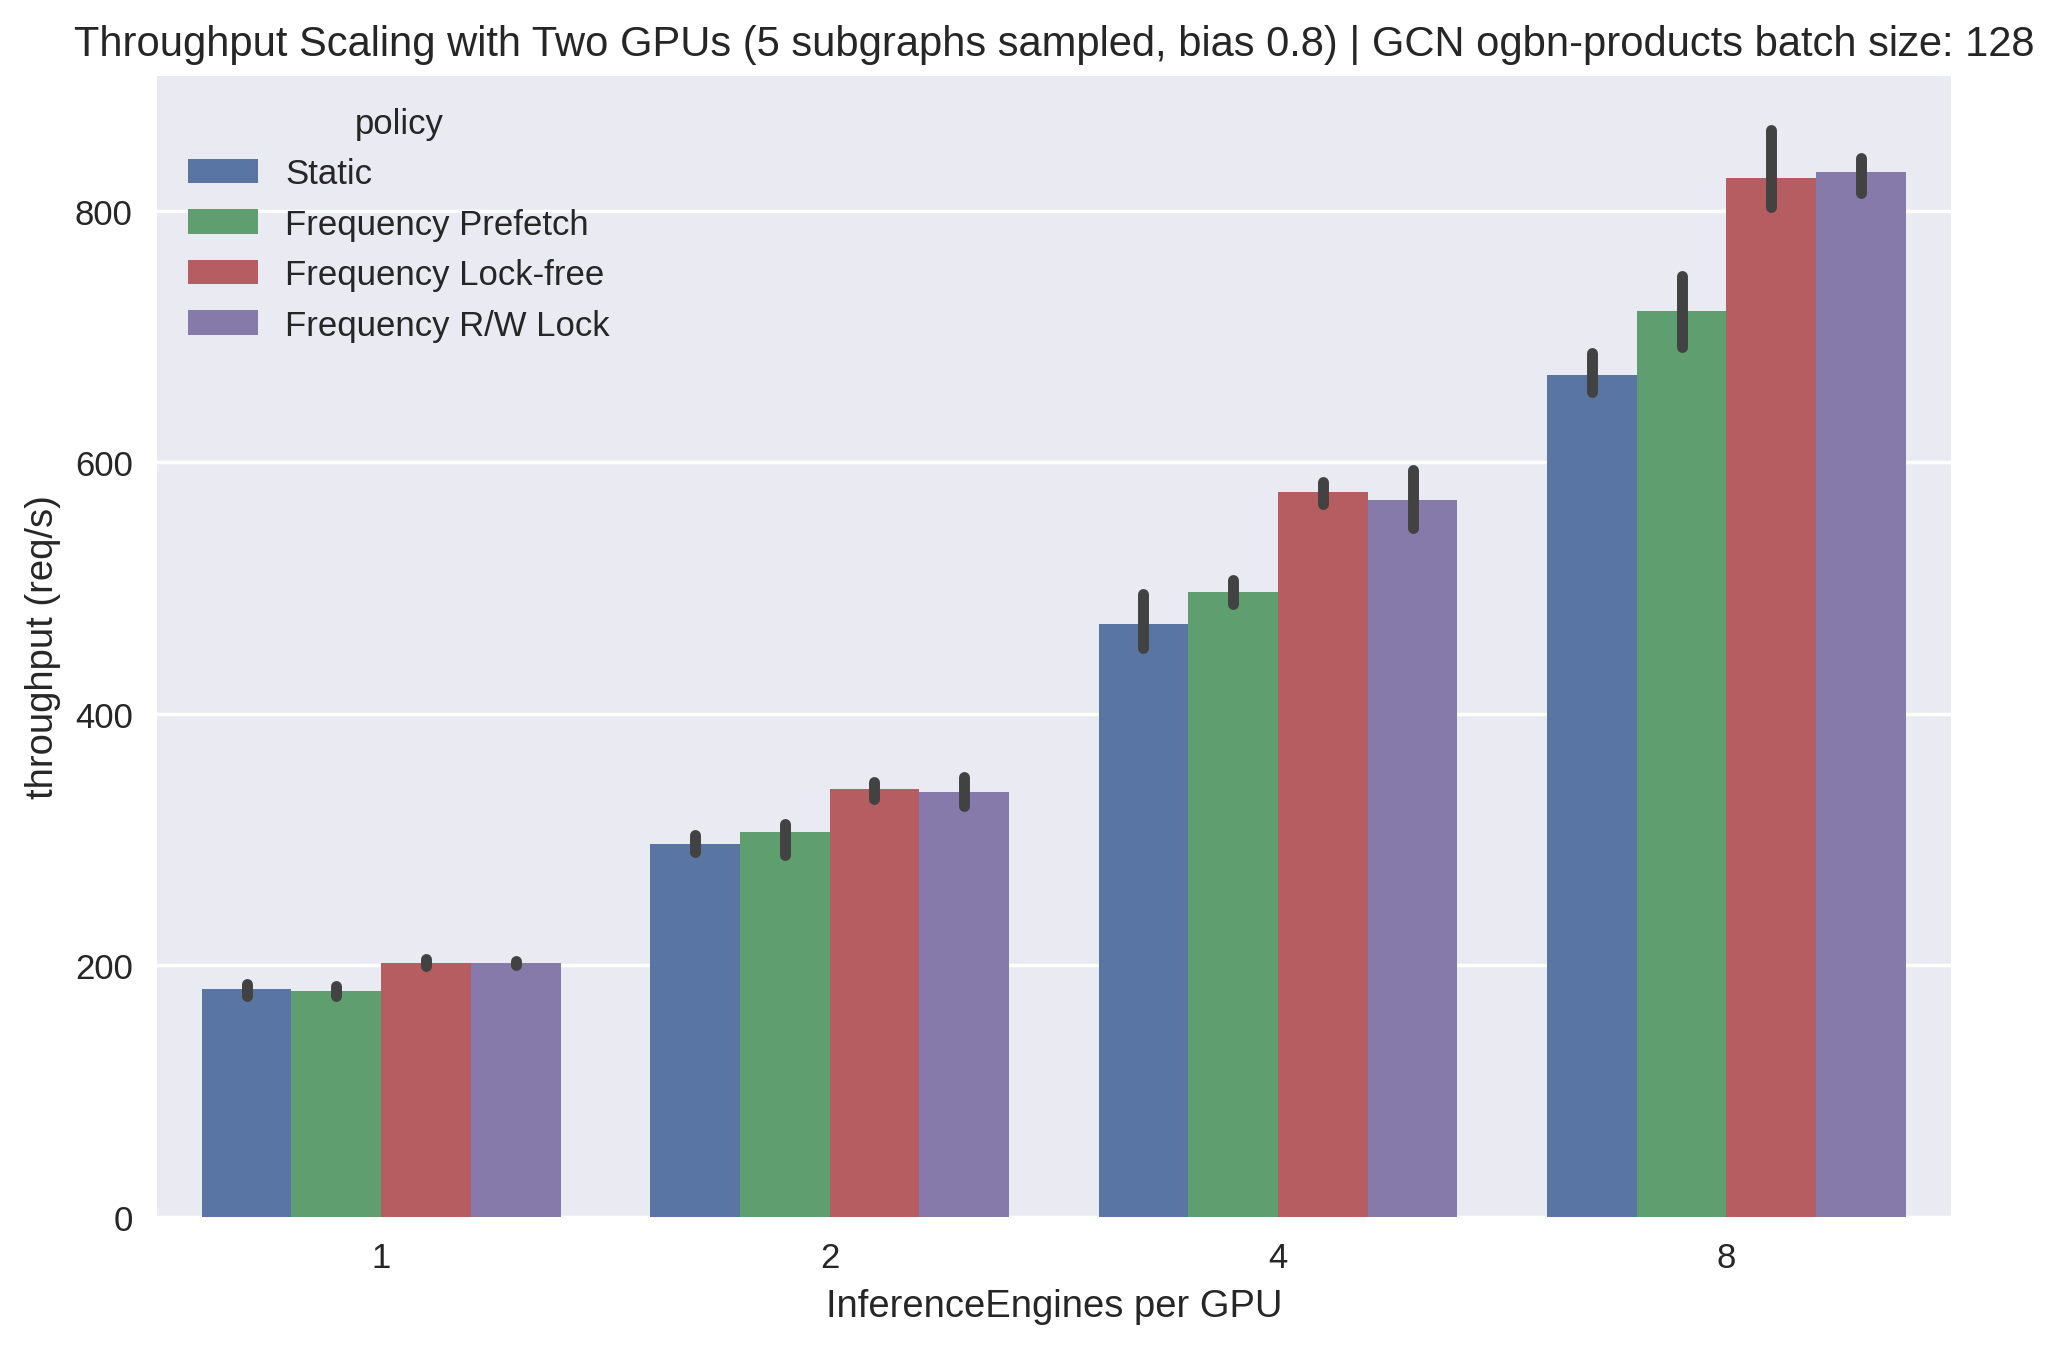
\includegraphics[width=\textwidth]{figures/throughput_GCN_bias_0.8_pinnedc0.2_gpus_2.png}
    \caption{[todo throughput]}
    \label{Eval: Latency speedup}
\end{figure}    

\subsection{Cache Hit Rate}
\begin{figure}[h!]
    \centering
    % 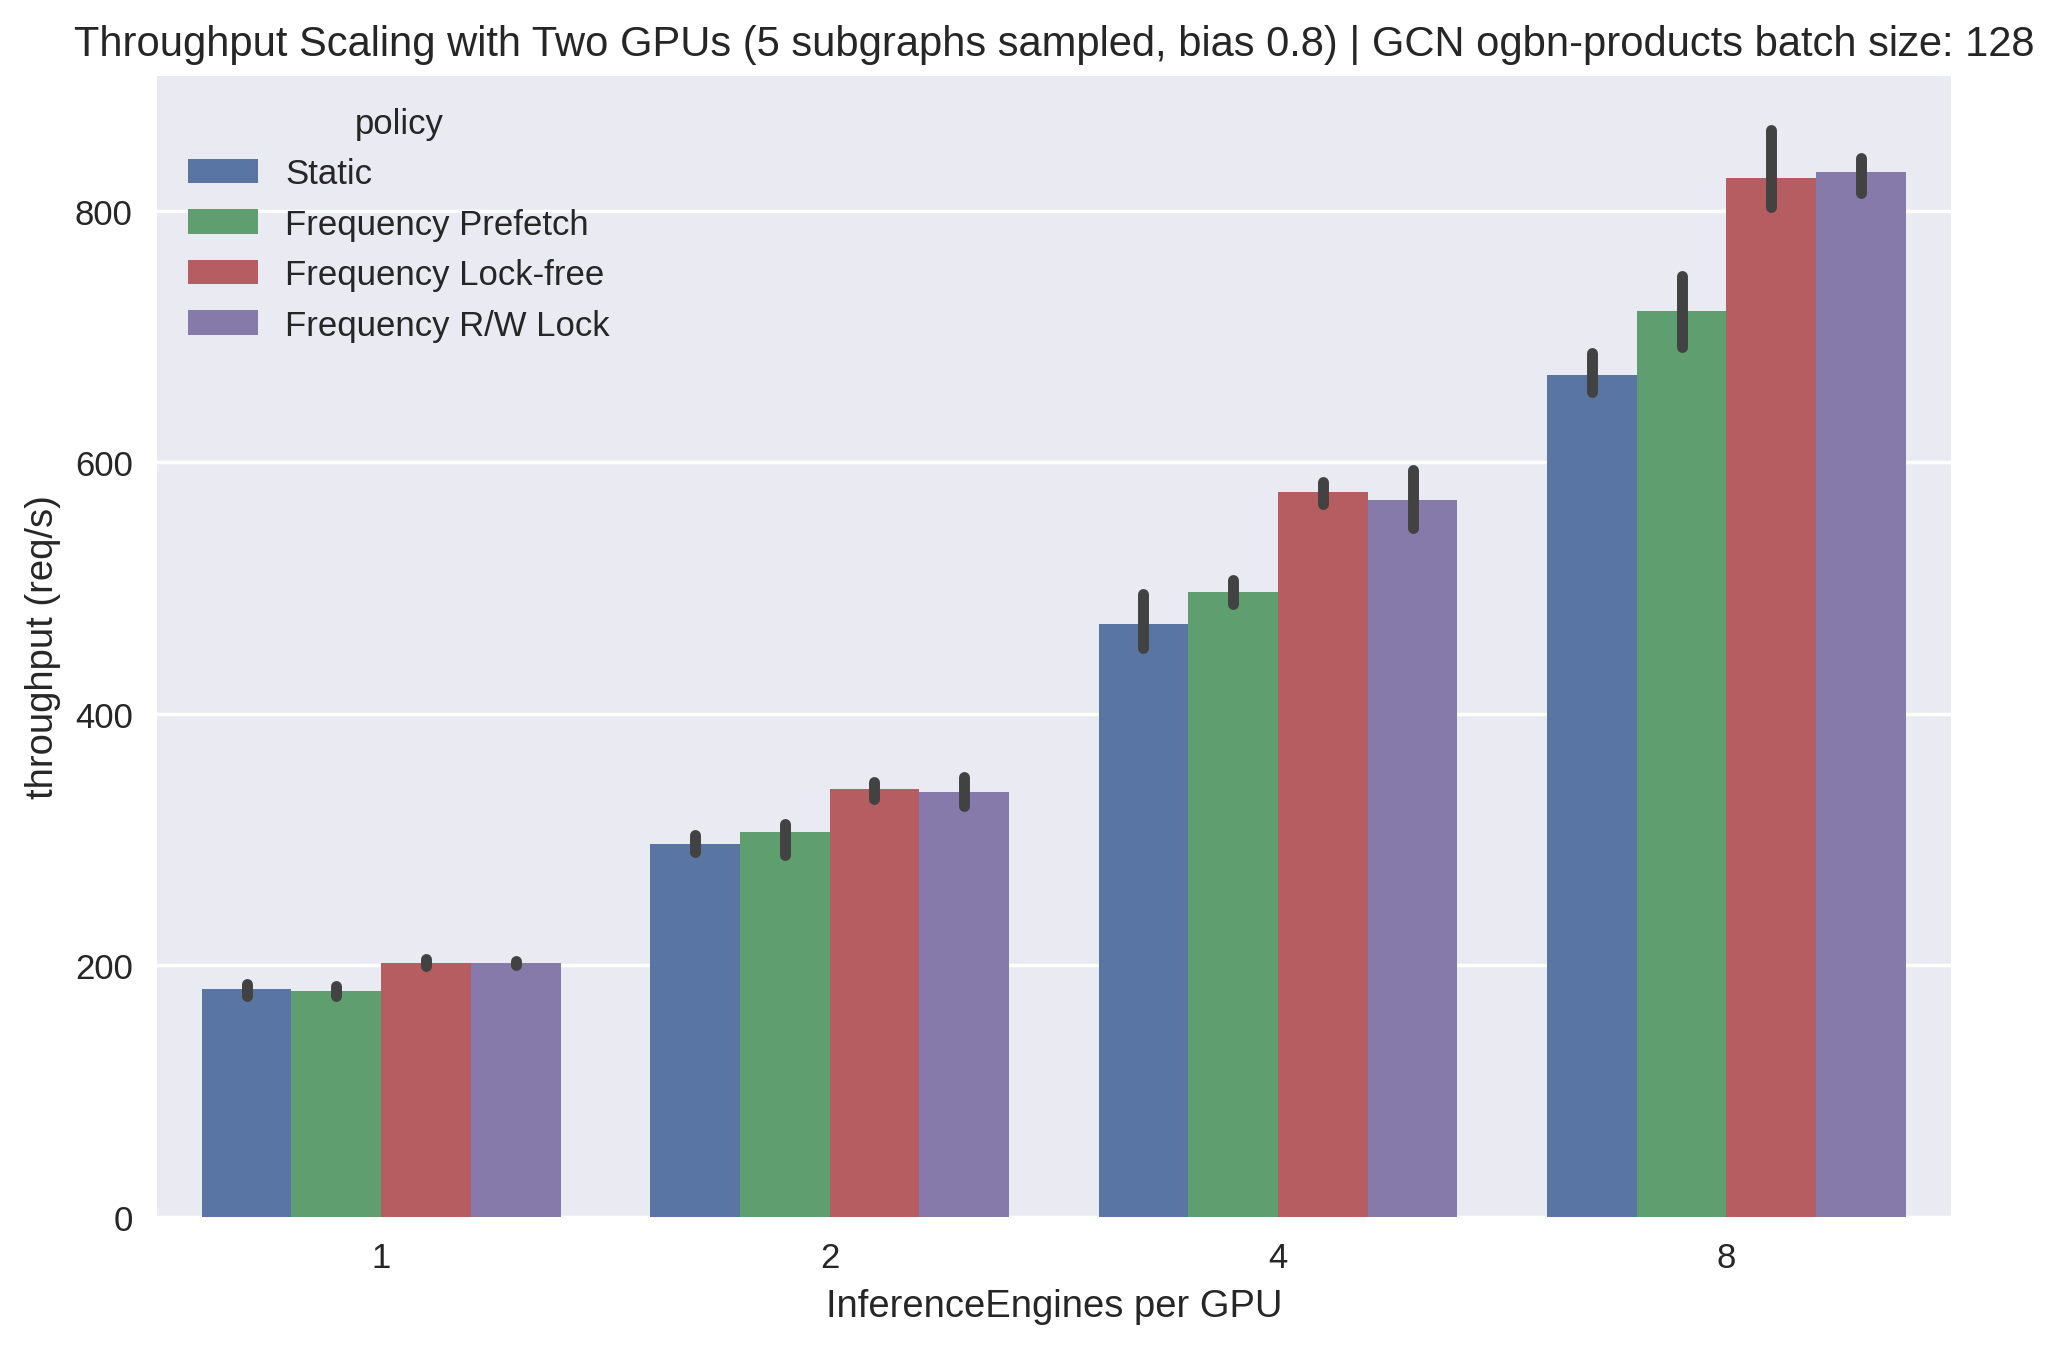
\includegraphics[width=\textwidth]{figures/throughput_GCN_bias_0.8_pinnedc0.2_gpus_2.png}
    \caption{[todo throughput]}
    \label{Eval: Hit Rate}
\end{figure}    
%%%%%%%%%%%%%%%%%%%%%%%%%%%%%%%%%%%%%%%%%%%%%%%%%%%%%%%%%%%%%%%%%%%%%%%%
\section{Locking vs. Lock-free}
%%%%%%%%%%%%%%%%%%%%%%%%%%%%%%%%%%%%%%%%%%%%%%%%%%%%%%%%%%%%%%%%%%%%%%%%

Figure \ref{Eval: Throughput} compares the throughput of our system using different cache replacement policies and mechanisms.

\subsection{Throughput}

\begin{figure}[h!]
    \centering
    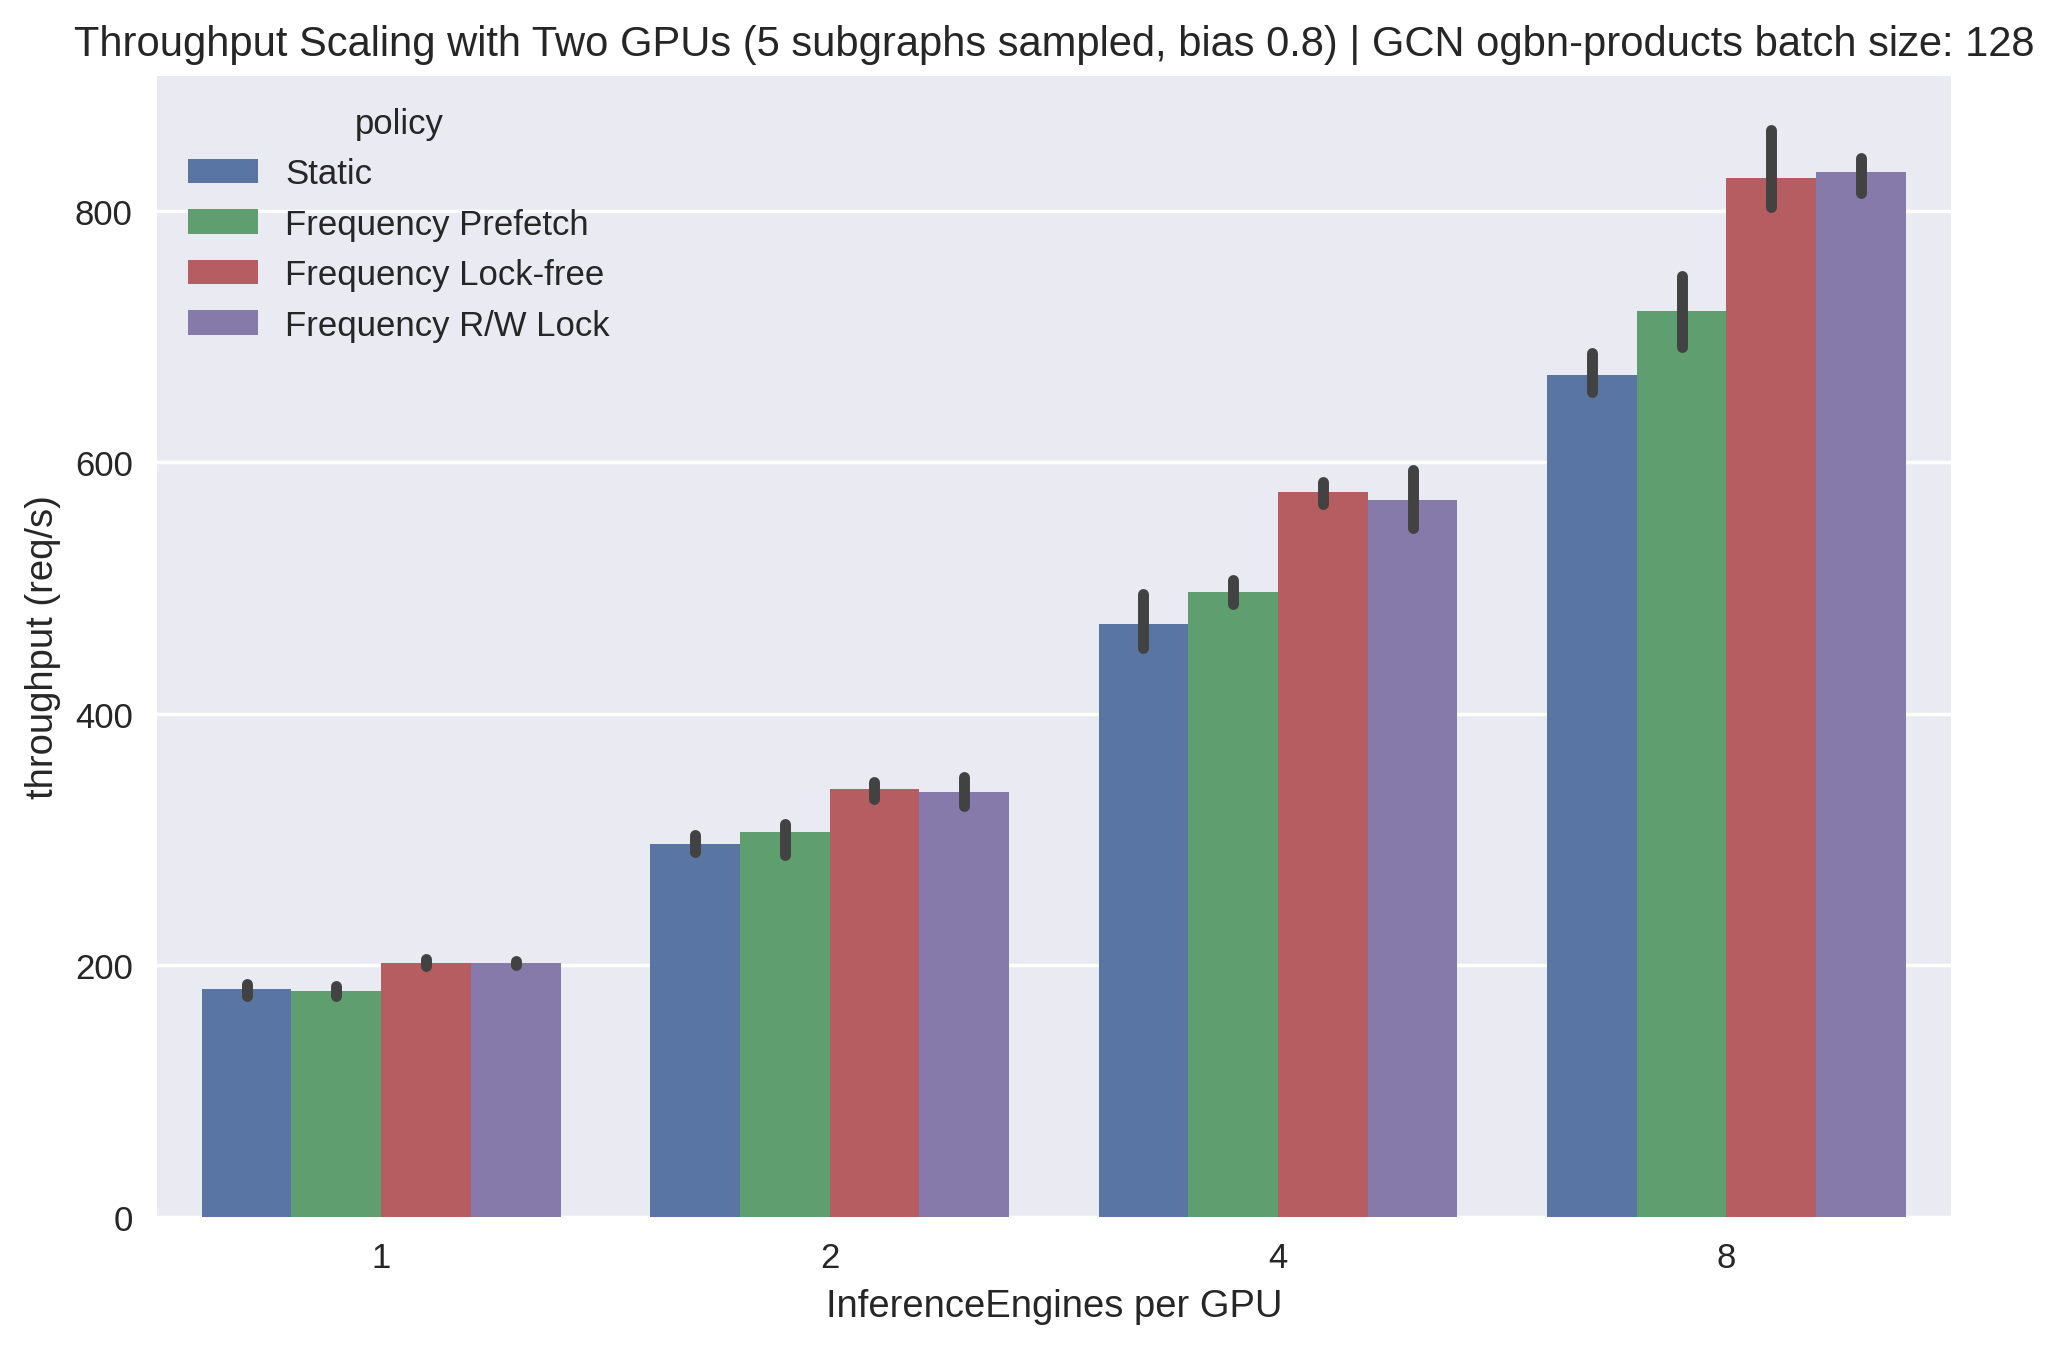
\includegraphics[width=0.8\textwidth]{figures/throughput_GCN_bias_0.8_pinnedc0.2_gpus_2.png}
    \caption{Peak throughput using two GPUs and varying number of InferenceEngines per GPU,}
    \label{Eval: Throughput}
\end{figure}    

Although there is little discernable difference in throughput between the lock-free and R/W lock approaches, there is an impact on P99 latency. Figure \ref{Eval: P99 latency} demonstrates these differences.
Note the log scale.

% \begin{figure}[h!]
%     \centering
%     % \includegraphics[width=\textwidth]{stamp_graphs.png}
    
%     \caption{[todo Lock conflict p99 latency]}
%     \label{Eval: P99 latency}
% \end{figure}    

To evaluate our system
\begin{figure}[h!]
    \centering
    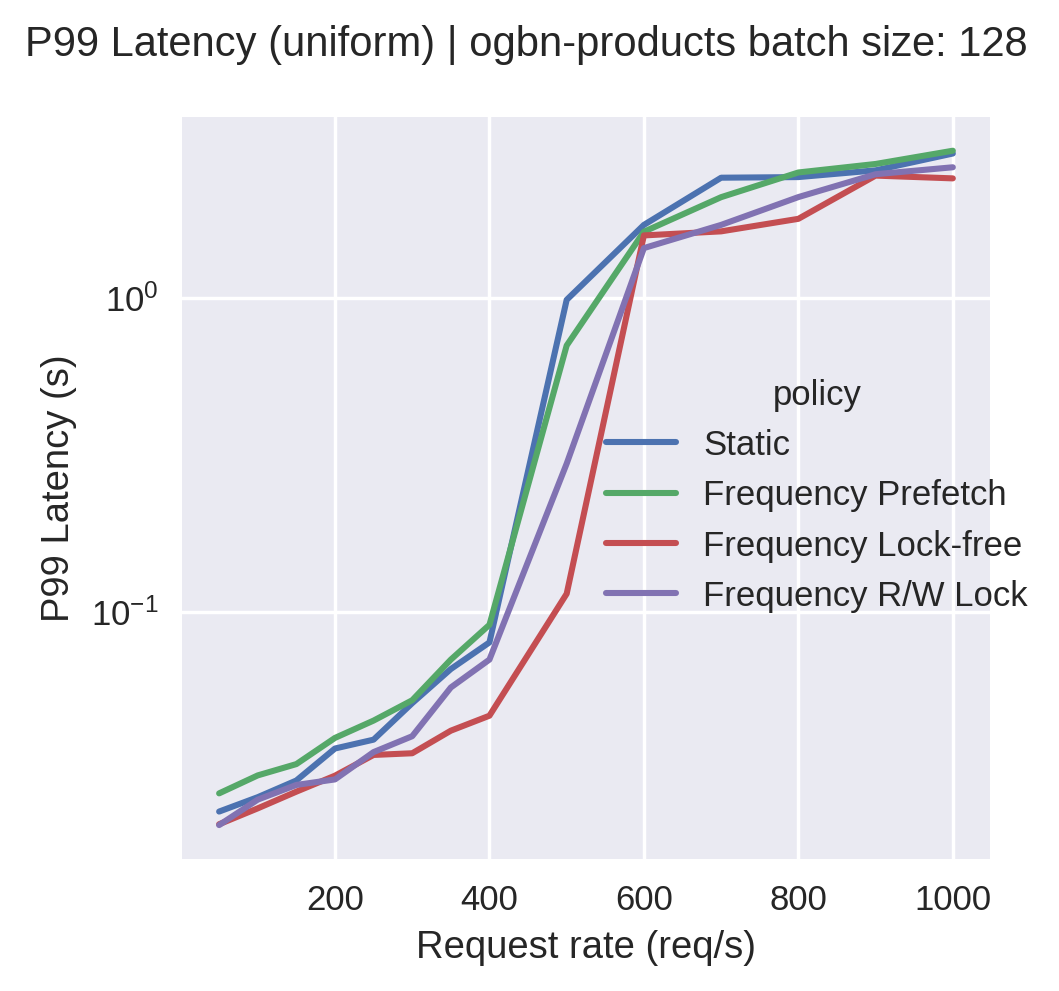
\includegraphics[width=0.85\textwidth]{figures/P99_latency_GCN_uniform_pinnedc0.2_gpus_3.png}    
    \caption{99\th percentile latencies for varying request rates. Tested on system using both GPUs and eight InferenceEngines per GPU.}
    \label{Eval: P99 latency}
\end{figure}  
Results are similar for the subgraph biased case.

\begin{figure}[h!]
    \centering
    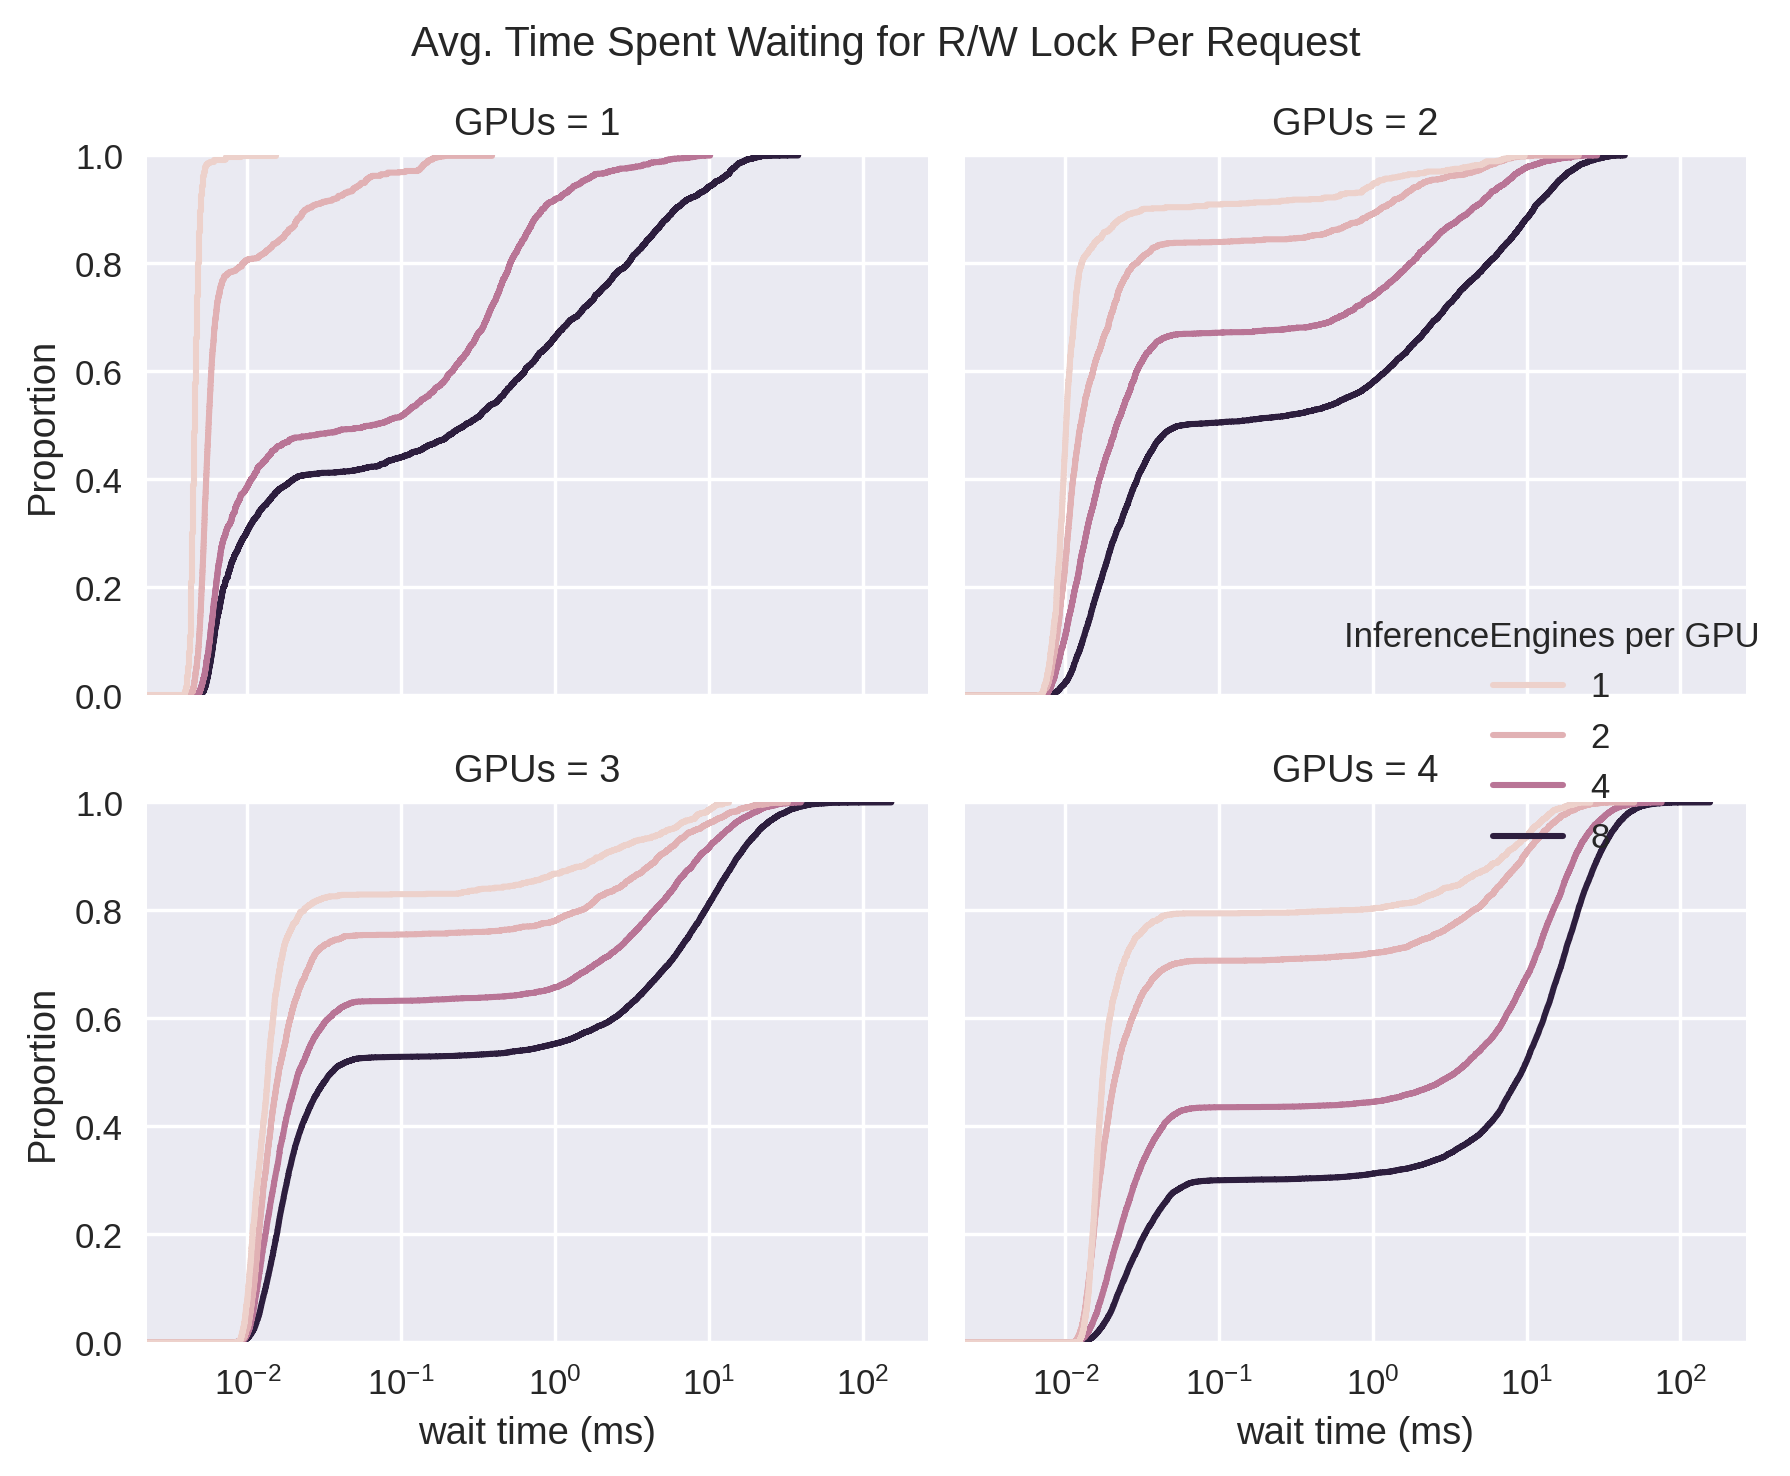
\includegraphics[width=\textwidth]{figures/Lock_Conflicts.png}
    
    \caption{[todo Lock conflict microbenchmark]}
    \label{Eval: Lock conflict microbenchmark}
\end{figure}    






%%%%%%%%%%%%%%%%%%%%%%%%%%%%%%%%%%%%%%%%%%%%%%%%%%%%%%%%%%%%%%%%%%%%%%%%
\section{PyTorch Direct Experiments}
%%%%%%%%%%%%%%%%%%%%%%%%%%%%%%%%%%%%%%%%%%%%%%%%%%%%%%%%%%%%%%%%%%%%%%%%
